\section{Match hypothesis}

Our implementation considers a simple match algorithm(brute force). For each keypoints of frame $i$ we find the closest match in the frame $i+1$ iterating over all possible candidates. We compare \textit{L2 Norm} and \textit{cosine} metrics to measure the similarity. Note that this implementation can generate the same match for two different keypoints yielding in an outlier.

An idea for performance improvement of this algorithm, is to use \textit{KNN(K-Nearest Neighbors)}. For real time application this may be a good option because its complexity is $O(n\log n)$, while our approach is $O(n^2)$ ($n$ is the number of keypoints).

Figure \ref{fig:diff-l2-cosine} shows the different result comparing \textit{L2 Norm} and \textit{cosine} metrics.


\begin{figure}[!h]
	\centering
	\begin{subfigure}{0.5\textwidth}
	  \centering
	  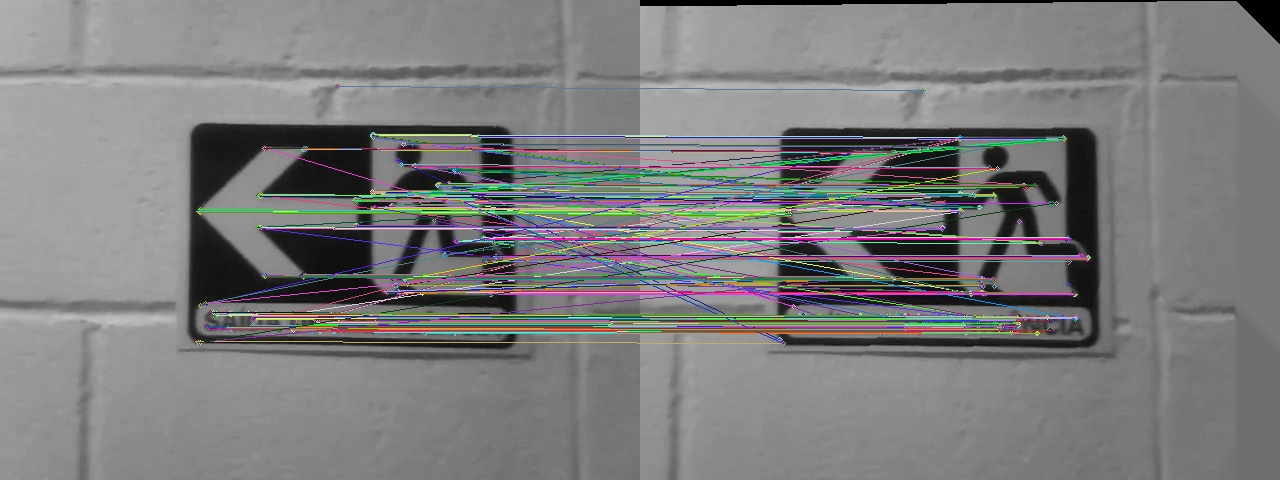
\includegraphics[width=0.9\linewidth]{figs/affine_100_cosine_30_8_False_p2-1-1_6-7.jpg}
	  \caption{Match hypothesis with cosine distance}
	\end{subfigure}%
	\begin{subfigure}{0.5\textwidth}
	  \centering
	  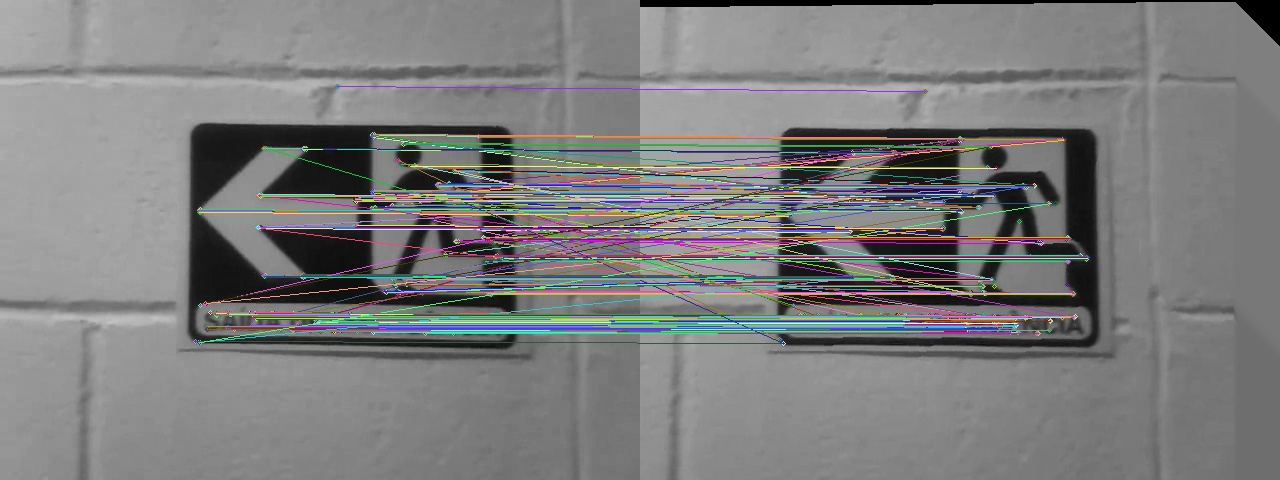
\includegraphics[width=0.9\linewidth]{figs/affine_200_l2-norm_30_8_False_p2-1-1_6-7.jpg}
	  \caption{Match hypothesis with l2-norm distance}
	\end{subfigure}
	\begin{subfigure}{0.5\textwidth}
        \centering
        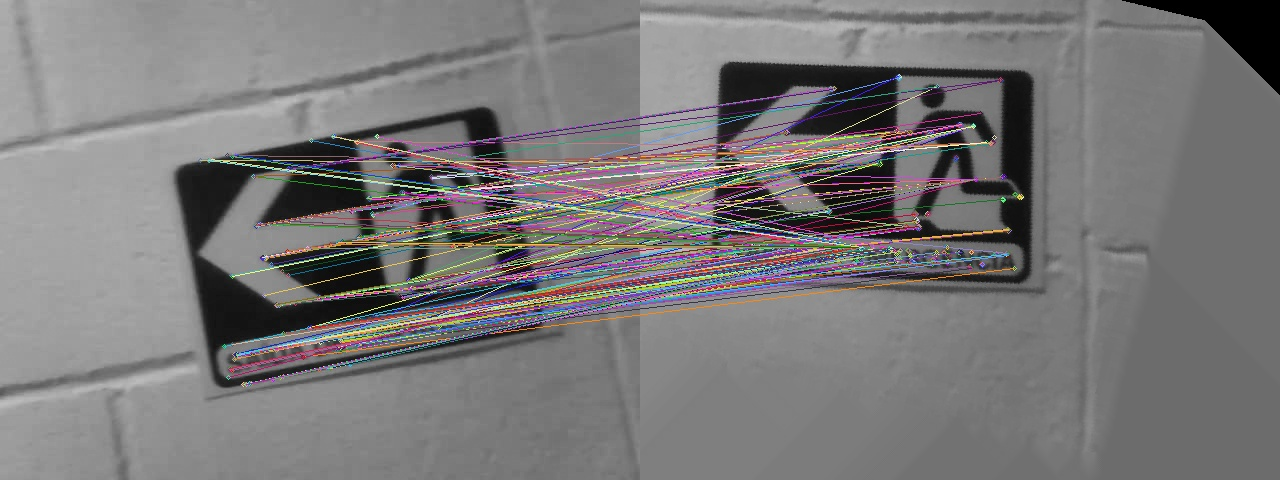
\includegraphics[width=0.9\linewidth]{figs/affine_100_cosine_30_8_False_p2-1-1_139-140.jpg}
        \caption{Match hypothesis with cosine distance}
      \end{subfigure}%
      \begin{subfigure}{0.5\textwidth}
        \centering
        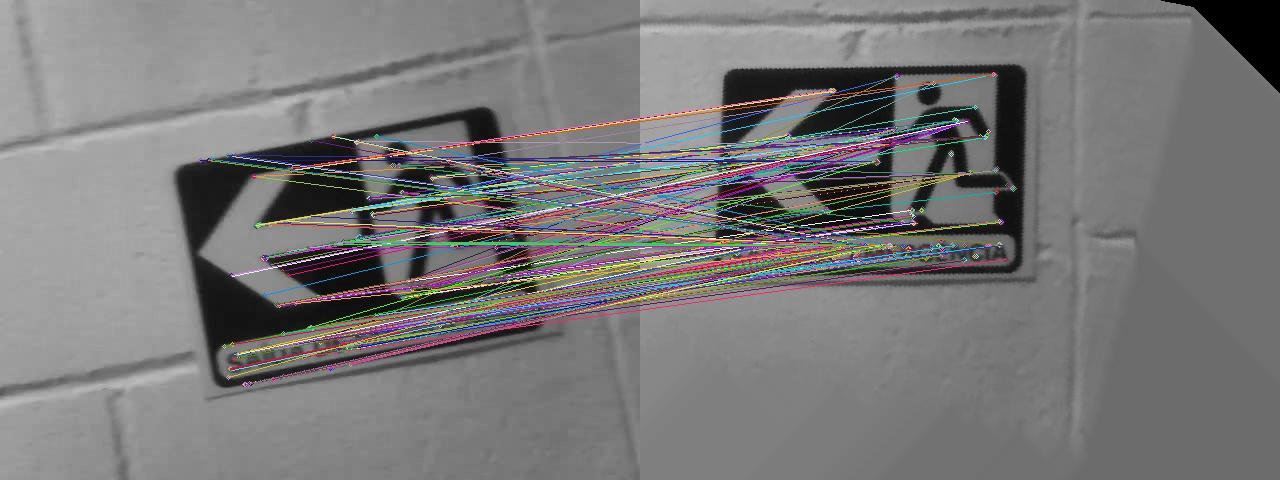
\includegraphics[width=0.9\linewidth]{figs/affine_200_l2-norm_30_8_False_p2-1-1_139-140.jpg}
        \caption{Match hypothesis with l2-norm distance}
      \end{subfigure}%
       \caption{Comparison of match hypothesis with cosine and l2-norm}
	\label{fig:diff-l2-cosine}
\end{figure}

We can see in figure ~\ref{fig:diff-l2-cosine} that the result of the experiment are very similar because there is not such an extreme difference between the performance of these metrics. There is an interesting difference in the execution time, as shown in table~\ref{table:dis-time}. L2-norm is slightly faster.  

\begin{table}[H]
\centering
\begin{tabular}{|l|c|c|}
\hline
\multicolumn{1}{|c|}{\multirow{2}{*}{\textbf{Name}}} & \multicolumn{2}{c|}{\textbf{Time per frame}} \\ \cline{2-3} 
\multicolumn{1}{|c|}{} & \textbf{L2-norm} & \textbf{Cosine} \\ \hline
p2-1-0.avi & 54.446 & 64.327 \\ \hline
p2-2-0.av & 37.321 & 42.982 \\ \hline
p2-2-0.avi & 54.446 & 45.262 \\ \hline
\end{tabular}
\caption{Execution time comparison.}
\label{table:dis-time}
\end{table}

We use \textit{cosine} distance as main similarity metric.
